\documentclass[11pt]{article}
\usepackage{a4wide}
\usepackage{latexsym}
\usepackage{amssymb}
\usepackage{epic}
\usepackage{graphicx}
%\pagestyle{empty}
\newcommand{\tr}{\mbox{\sf true}}
\newcommand{\fa}{\mbox{\sf false}}
\newcommand{\bimp}{\leftrightarrow}


\begin{document}

\section*{
\begin{center}
Practical Assignment Part 1\\
Automated Reasoning 2IMF25\\
\end{center}
}

\begin{center}
Technische Universiteit Eindhoven\\
Jiahuan Zhang (j.4.zhang@student.tue.nl)\\
Hector Joao Rivera Verduzco (h.j.rivera.verduzco@student.tue.nl)\\

\end{center}
\date{\today}
\vspace{5mm}

\subsection*{Problem 1}

Six trucks have to deliver pallets of obscure building blocks to a magic factory. Every truck has a capacity of 7800 kg and can carry at most eight pallets. In total, the following has to be delivered:
\begin{itemize}
  \item Four pallets of nuzzles, each of weight 700 kg.
  \item A number of pallets of prittles, each of weight 800 kg.
  \item Eight pallets of skipples, each of weight 1000 kg.
  \item Ten pallets of crottles, each of weight 1500 kg.
  \item Five pallets of dupples, each of weight 100 kg.
\end{itemize}
Prittles and crottles are an explosive combination: they are not allowed to be put in the same truck.\\
Skipples need to be cooled; only two of the six trucks have facility for cooling skipples.\\
Dupples are very valuable; to distribute the risk of loss no two pallets of dupples may be in the same truck.\\
Investigate what is the maximum number of pallets of prittles that can be delivered, and show how for that number all pallets may be divided over the six trucks.

\vspace{4mm}

\subsection*{Solution:}

We generalize this problem so that truck Nr. $i$ delivers pallets of obscure building blocks labeled $j$, $1\leq i \leq6$ and $1\leq j \leq5$.

Then we introduce $t_{ij}$ as a nature number, which represents the number of pallets of obscure building block $j$ on truck Nr. $i$.
\begin{center}
\begin{tabular}{|c|c|c|c|c|c|}
  \hline
  % after \\: \hline or \cline{col1-col2} \cline{col3-col4} ...
    & nuzzles & prittles & skipples & crottles & dupples \\
  $j$ & 1 & 2 & 3 & 4 & 5 \\
  $weight(j)$ & 700kg & 800kg & 1000kg & 1500kg & 100kg \\
  $NROFpallets(j)$ & 4 & $n$ & 8 & 10 & 5 \\
  \hline
\end{tabular}
\end{center}

Now we consider the conditions for the delivery.

\begin{description}
  \item[Condition 1:] $t_{ij}$ should be no less than $0$.

  This is expressed by the formula
  \[ \bigwedge_{i,j:1 \leq i \leq 6, 1 \leq j \leq 5} t_{ij} \geq 0.\]
  \item[Condition 2:] Every truck has a capacity of 7800 kg.

  \[ \bigwedge_{i=1}^6  (\sum_{j=1}^5 t_{ij} \times weight(j)) \leq 7800 .\]
  \item[Condition 3:] Every truck can carry at most eight pallets.

  \[ \bigwedge_{i=1}^6 (\sum_{j=1}^5 t_{ij}) \leq 8 .\]
  \item[Condition 4:] Except for prittles, the sum of the pallets of the other obscure building blocks should be exact the same as the given number.

  \[ \bigwedge_{1\leq j \leq5, j\neq2} (\sum_{i=1}^6 t_{ij}) = NROFpallets(j) .\]
  \item[Condition 5:] We are required to find out the maximum number of the pallets of prittles.

  First find out the possible maximum number of it. Since we know the capacity of each track and the total weights of the pallets of the other obscure building blocks, we can estimate the number.

  $\frac{7800 \times 6 - 700\times4 - 1000\times8 - 1500\times10 - 100\times5}{800} = 25.625$

  Because the number of pallet is a nature number, the maximum number should not be more than 25. Therefore, we can stop the debugging until $n = 25$.

  $\sum_{i=1}^6 t_{i2}) \leq 25$
  \item[Condition 6:] Prittles and crottles are not allowed to be put in the same truck.

  \[ \bigwedge_{i=1}^6 t_{i2}=0 \vee t_{i4}=0 .\]
  \item[Condition 7:] Only two of the six trucks can deliver skipples.

  \[ \bigvee_{i,k:1 \leq i < k \leq 6} t_{i3} + t_{k3} = 8 .\]
  \item[Condition 8:] No two pallets of dupples may be in the same truck.

  \[ \bigwedge_{i=1}^6 t_{i5} \leq 1 .\]
\end{description}

The total formula now consists of the conjunction of all these
ingredients, that is,
\[ \bigwedge_{i,j:1 \leq i \leq 6, 1 \leq j \leq 5} t_{ij} \geq 0 \;\; \wedge \]
\[ \bigwedge_{i=1}^6  (\sum_{j=1}^5 t_{ij} \times weight(j)) \leq 7800 \;\; \wedge \]
\[ \bigwedge_{i=1}^6 (\sum_{j=1}^5 t_{ij}) \leq 8 \;\; \wedge \]
\[ \bigwedge_{1\leq j \leq5, j\neq2} (\sum_{i=1}^6 t_{ij}) = NROFpallets(j) \;\; \wedge \]
\[ \sum_{i=1}^6 t_{i2}) \leq 25 \;\; \wedge \]
\[ \bigwedge_{i=1}^6 t_{i2}=0 \vee t_{i4}=0 \;\; \wedge \]
\[ \bigvee_{i,k:1 \leq i < k \leq 6} t_{i3} + t_{k3} = 8 \;\; \wedge \]
\[ \bigwedge_{i=1}^6 t_{i5} \leq 1 \]

This formula is easily expressed in SMT syntax.

{\footnotesize

{\tt (benchmark Part1\_1.smt}

{\tt :logic $QF\_ALIA$}

{\tt :extrafuns (}

{\tt (t11 Int) (t12 Int) (t13 Int) (t14 Int) (t15 Int) }

{\tt (t21 Int) (t22 Int) (t23 Int) (t24 Int) (t25 Int) }

{\tt (t31 Int) (t32 Int) (t33 Int) (t34 Int) (t35 Int) }

{\tt (t41 Int) (t42 Int) (t43 Int) (t44 Int) (t45 Int) }

{\tt (t51 Int) (t52 Int) (t53 Int) (t54 Int) (t55 Int) }

{\tt (t61 Int) (t62 Int) (t63 Int) (t64 Int) (t65 Int) }

{\tt )}

{\tt :formula}

{\tt   (and}

{\tt (>= t11 0) (>= t12 0) (>= t13 0) (>= t14 0) (>= t15 0)}

{\tt (>= t21 0) (>= t22 0) (>= t23 0) (>= t24 0) (>= t25 0)}

$\cdots \cdots$

{\tt (>= t61 0) (>= t62 0) (>= t63 0) (>= t64 0) (>= t65 0) }

{\tt (<= (+ (* t11 700) (* t12 1300) (* t13 1000) (* t14 1500) (* t15 100)) 7800)}

{\tt (<= (+ (* t21 700) (* t22 1300) (* t23 1000) (* t24 1500) (* t25 100)) 7800)}

{\tt (<= (+ (* t31 700) (* t32 1300) (* t33 1000) (* t34 1500) (* t35 100)) 7800)}

{\tt (<= (+ (* t41 700) (* t42 1300) (* t43 1000) (* t44 1500) (* t45 100)) 7800)}

{\tt (<= (+ (* t51 700) (* t52 1300) (* t53 1000) (* t54 1500) (* t55 100)) 7800)}

{\tt (<= (+ (* t61 700) (* t62 1300) (* t63 1000) (* t64 1500) (* t65 100)) 7800) }

{\tt (<= (+ t11 t12 t13 t14 t15) 8)}

{\tt (<= (+ t21 t22 t23 t24 t25) 8)}

{\tt (<= (+ t31 t32 t33 t34 t35) 8)}

{\tt (<= (+ t41 t42 t43 t44 t45) 8)}

{\tt (<= (+ t51 t52 t53 t54 t55) 8)}

{\tt (<= (+ t61 t62 t63 t64 t65) 8)}

{\tt (= (+ t11 t21 t31 t41 t51 t61) 4)}

{\tt (<= (+ t12 t22 t32 t42 t52 t62) 25)}

{\tt (>= (+ t12 t22 t32 t42 t52 t62) 15)}

{\tt (= (+ t13 t23 t33 t43 t53 t63) 8)}

{\tt (= (+ t14 t24 t34 t44 t54 t64) 10)}

{\tt (= (+ t15 t25 t35 t45 t55 t65) 5)}

{\tt (or (= t12 0) (= t14 0)) }

{\tt (or (= t22 0) (= t24 0)) }

{\tt (or (= t32 0) (= t34 0)) }

{\tt (or (= t42 0) (= t44 0)) }

{\tt (or (= t52 0) (= t54 0)) }

{\tt (or (= t62 0) (= t64 0)) }

{\tt (or}

{\tt (= (+ t13 t23) 8) (= (+ t13 t33) 8) (= (+ t13 t43) 8) (= (+ t13 t53) 8) }

{\tt (= (+ t13 t63) 8) (= (+ t23 t33) 8) (= (+ t23 t43) 8) (= (+ t23 t53) 8) }

{\tt (= (+ t23 t63) 8) (= (+ t33 t43) 8) (= (+ t33 t53) 8) (= (+ t33 t63) 8) }

{\tt (= (+ t43 t53) 8) (= (+ t43 t63) 8) (= (+ t53 t63) 8)) }

{\tt (<= t15 1) (<= t25 1) (<= t35 1) (<= t45 1) (<= t55 1) (<= t65 1)}

{\tt )) }
}

Applying {\tt yices-smt -m Part1\_1.smt} several time, we find when the number of pallets of prittles is 16, it is UNSAT. When the number is 15, it is SAT. Therefore, we conclude that the maximal number of pallets of prittles is 15.
The following result is yielded within a fraction of a second:

\begin{center}
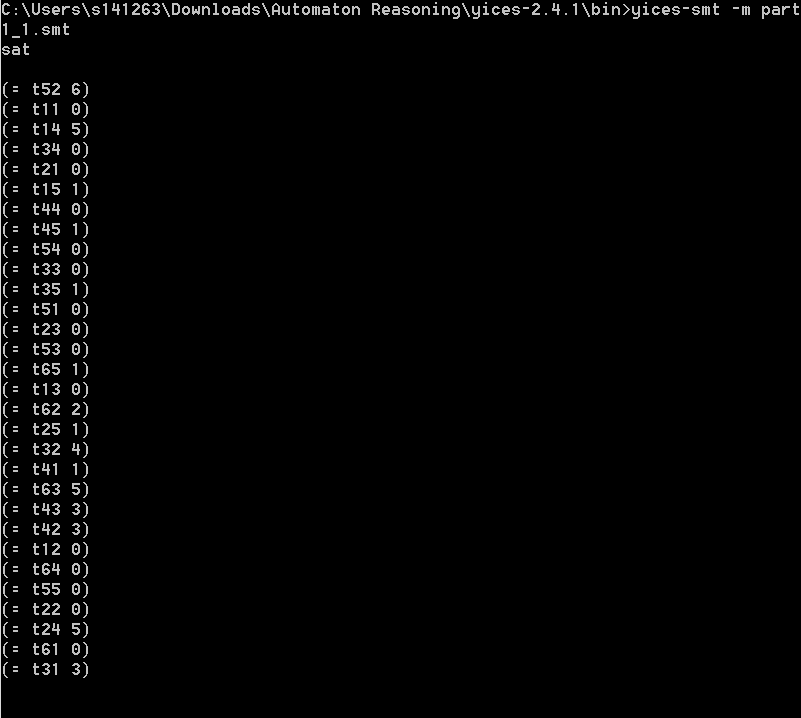
\includegraphics[width=1.0\textwidth]{Part1_1.png}
\end{center}

\vspace{3mm}

{\bf Remark:}

\vspace{3mm}

{\bf Generalization:}


\vspace{5mm}

\subsection*{Problem 2}

Give a chip design containing three power components and eight regular components satisfying the following constraints:
\begin{itemize}
  \item The width of the chip is 29 and the height is 22.
  \item All power components have width 4 and height 2.
  \item The sizes of the eight regular components are $9 \times 7$, $12 \times 6$, $10 \times 7$, $18 \times 5$, $20 \times 4$, $10 \times 6$, $8 \times 6$ and $10 \times 8$, respectively.
  \item All components may be turned 90±, but may not overlap.
  \item In order to get power, all regular components should directly be connected to a power component, that is, an edge of the component should have at least one point in common with an edge of the power component.
  \item Due to limits on heat production the power components should be not too close: their centres should differ at least 17 in either the x direction or the y direction (or both).
\end{itemize}

\vspace{4mm}

\subsection*{Solution:}

\vspace{3mm}

{\bf Remark:}

\vspace{3mm}

{\bf Generalization:}

\vspace{5mm}

\subsection*{Problem 3}

Twelve jobs numbered from 1 to 12 have to be executed satisfying the following requirements:
\begin{itemize}
  \item The running time of job $i$ is $i$, for $i = 1, 2, . . . , 12$.
  \item All jobs run without interrupt.
  \item Job 3 may only start if jobs 1 and 2 have been finished.
  \item Job 5 may only start if jobs 3 and 4 have been finished.
  \item Job 7 may only start if jobs 3, 4 and 6 have been finished.
  \item Job 9 may only start if jobs 5 and 8 have been finished.
  \item Job 11 may only start if Job 10 has been finished.
  \item Job 12 may only start if jobs 9 and 11 have been finished.
  \item Jobs 5,7 en 10 require a special equipment of which only one copy is available, so no two of these jobs may run at the same time.
\end{itemize}
Find a solution of this scheduling problem for which the total running time is minimal.

\vspace{4mm}

\subsection*{Solution:}
First we introduce two variables $S_{i}$ and $D_{i}$ for $i = 1,2,3,...,12$.
\begin{itemize}
  \item $S_{i}$ is the starting time of Job $i$. $S_{i} \geq 0$. For example: Job 1 starts at 0, then $S_{1} = 0$. $S_{i}$ can be any positive integer number if it is satisfied with all requirements.
  \item $D_{i}$ is the duration of Job $i$. For example: the running time of Job 1 is 1, then $D_{1} = 1$. $D_{i}$ is a fixed integer number.
\end{itemize}

Secondly, we find the clauses which have to be satisfied by  all requirements of this problem.

\begin{description}
  \item[Requirement 1:] The running time of job $i$ is $i$, for $i = 1, 2, . . . , 12$.

  So we have 
  
  $D_{1}=1$ , $D_{2}=2$, $D_{3}=3$, $D_{4}=4$, $D_{5}=5$, $D_{6}=6$, 
  
  $D_{7}=7$, $D_{8}=8$, $D_{9}=9$, $D_{10}=10$, $D_{11}=11$ and $D_{12}=12$.
  \item[Requirement 2:] All jobs run without interrupt.

  Thus, we are able to define the total time consumed by each job. \\
    \begin{center}
    The total time for Job 1 is $S_{1}+D_{1}=S_{1}+1$.\\
    The total time for Job 2 is $S_{2}+D_{2}=S_{2}+2$.\\
    The total time for Job 3 is $S_{3}+D_{3}=S_{3}+3$.\\
    $\vdots$\\
    The total time for Job 12 is $S_{12}+D_{12}=S_{12}+12$.
    \end{center}
  \item[Requirement 3:] Job 3 may only start if jobs 1 and 2 have been finished.

  So we have
  \begin{center}
  if $(S_{1}+D_{1}) \geq (S_{2}+D_{2})$, then $S_{3} \geq (S_{1}+D_{1})$.\\
  if $(S_{2}+D_{2}) \geq (S_{2}+D_{2})$, then $S_{3} \geq (S_{2}+D_{2})$.
  \end{center}
  Translating this requirement into Yices code, we have
  \begin{center}
  {\tt (ite (>= (+ s1 d1) (+ s2 d2)) (>= s3 (+ s1 d1)) (>= s3 (+ s2 d2)))}
  \end{center}
  Denote the codes as Clause $A$.
  \item[Requirement 4:] Job 5 may only start if jobs 3 and 4 have been finished.

  So we have
  \begin{center}
  if $(S_{3}+D_{3}) \geq (S_{4}+D_{4})$, then $S_{5} \geq (S_{3}+D_{3})$.\\
  if $(S_{4}+D_{4}) \geq (S_{3}+D_{3})$, then $S_{5} \geq (S_{4}+D_{4})$.
  \end{center}
  Translating this requirement into Yices code, we have
  \begin{center}
  {\tt (ite (>= (+ s3 d3) (+ s4 d4)) (>= s5 (+ s3 d3)) (>= s5 (+ s4 d4)))}
  \end{center}
  Denote the codes as Clause $B$.
  \item[Requirement 5:] Job 7 may only start if jobs 3, 4 and 6 have been finished.

  Using the same method as requirements 1 and 2, we get the following Yices codes.
  \begin{center}
  {\tt (ite (and (>= (+ s3 d3) (+ s4 d4)) (>= (+ s4 d4) (+ s6 d6))) (>= s7 (+ s3 d3) ) (>= s7 (+ s6 d6)))}

  {\tt (ite (and (>= (+ s3 d3) (+ s6 d6)) (>= (+ s6 d6) (+ s4 d4))) (>= s7 (+ s3 d3) ) (>= s7 (+ s4 d4)))}

  {\tt (ite (and (>= (+ s4 d4) (+ s3 d3)) (>= (+ s3 d3) (+ s6 d6))) (>= s7 (+ s4 d4) ) (>= s7 (+ s6 d6)))}

  {\tt (ite (and (>= (+ s4 d4) (+ s6 d6)) (>= (+ s6 d6) (+ s3 d3))) (>= s7 (+ s4 d4) ) (>= s7 (+ s3 d3)))}

  {\tt (ite (and (>= (+ s6 d6) (+ s3 d3)) (>= (+ s3 d3) (+ s4 d4))) (>= s7 (+ s6 d6) ) (>= s7 (+ s4 d4)))}

  {\tt (ite (and (>= (+ s6 d6) (+ s4 d4)) (>= (+ s4 d4) (+ s3 d3))) (>= s7 (+ s6 d6) ) (>= s7 (+ s3 d3)))}
  \end{center}
  The formula for this requirement is the conjunction of the codes above. Then we denote this conjunction as Clause $C$.
  \item[Requirement 6:] Job 9 may only start if jobs 5 and 8 have been finished.

  Using the same method as requirements 1 and 2, we get the following Yices code.
  \begin{center}
  {\tt (ite (>= (+ s5 d5) (+ s8 d8)) (>= s9 (+ s5 d5)) (>= s9 (+ s8 d8 )))}
  \end{center}
  Denote the codes as Clause $D$.
  \item[Requirement 7:] Job 11 may only start if Job 10 has been finished.

  \begin{center}
  {\tt (ite (>= (+ s5 d5) (+ s8 d8)) (>= s9 (+ s5 d5)) (>= s9 (+ s8 d8 )))}
  \end{center}
  Denote the codes as Clause $E$.
  \item[Requirement 8:] Job 12 may only start if jobs 9 and 11 have been finished.

  This requirement means that the starting time of Job 11 is bigger or equal to the total time for Job 10.
  Then we have the Yices codes as the follows.
  \begin{center}
  {\tt (>= s11 (+ s10 d10))}
  \end{center}
  Denote the codes as Clause $F$.
  \item[Requirement 9:] Jobs 5,7 en 10 require a special equipment of which only one copy is available, so no two of these jobs may run at the same time.

  There are 6 possible orderings to sort Job 5, Job 7 and Job10. They are
  
  Job5$\rightarrow$Job7$\rightarrow$Job10: 
  
  {\tt (and (>= s5 0) (>= s7 (+ s5 d5)) (>= s10 (+ s5 s7 d5 d7)))}

  Job5$\rightarrow$Job10$\rightarrow$Job7: 
  
  {\tt (and (>= s5 0) (>= s10 (+ s5 d5)) (>= s7 (+ s5 s10 d5 d10)))}

  Job7$\rightarrow$Job5$\rightarrow$Job10: 
  
  {\tt (and (>= s7 0) (>= s5 (+ s7 d7)) (>= s10 (+ s5 s7 d5 d7)))}

  Job7$\rightarrow$Job10$\rightarrow$Job5: 
  
  {\tt (and (>= s7 0) (>= s10 (+ s7 d7)) (>= s5 (+ s10 s7 d10 d7)))}

  Job10$\rightarrow$Job5$\rightarrow$Job7: 
  
  {\tt (and (>= s10 0) (>= s5 (+ s10 d10)) (>= s7 (+ s5 s10 d5 d10)))}

  Job10$\rightarrow$Job7$\rightarrow$Job5: 
  
  {\tt (and (>= s10 0) (>= s7 (+ s10 d10)) (>= s5 (+ s10 s7 d10 d7)))}
  
  Take the disjunction of the codes for the orderings above and denote the disjunction as Clause G.
\end{description}
The total formula now consists of the conjunction of all these requirements.
\begin{center}
$A \bigwedge B \bigwedge C \bigwedge D \bigwedge E \bigwedge F \bigwedge G$
\end{center}
The complete formula expressed in SMT syntax is in the following.

{\tt (benchmark part1$\_$3}

{\tt :logic $QF\_ALIA$}

{\tt :extrafuns (}

{\tt (s1 Int) (s2 Int) (s3 Int) (s4 Int) (s5 Int) (s6 Int)}

{\tt (s7 Int) (s8 Int) (s9 Int) (s10 Int) (s11 Int) (s12 Int)}

{\tt (d1 Int) (d2 Int) (d3 Int) (d4 Int) (d5 Int) (d6 Int)}

{\tt (d7 Int) (d8 Int) (d9 Int) (d10 Int) (d11 Int) (d12 Int))}

{\tt :formula (and}

{\tt (>= s1 0) (>= s2 0) (>= s3 0) (>= s4 0) (>= s5 0) (>= s6 0))}

{\tt (>= s7 0) (>= s8 0) (>= s9 0) (>= s10 0) (>= s11 0) (= s12 24)}

{\tt (= d1 1) (= d2 2) (= d3 3) (= d4 4) (= d5 5) (= d6 6)}

{\tt (= d7 7) (= d8 8) (= d9 9) (= d10 10) (= d11 11) (= d12 12)}

{\tt (ite (>= (+ s1 d1) (+ s2 d2))  (>= s3 (+ s1 d1))  (>= s3 (+ s2 d2 )))}

{\tt (ite (>= (+ s3 d3) (+ s4 d4))  (>= s5 (+ s3 d3))  (>= s5 (+ s4 d4 )))}

{\tt (ite (and (>= (+ s3 d3) (+ s4 d4)) (>= (+ s4 d4) (+ s6 d6))) }

{\tt (>= s7 (+ s3 d3) ) (>= s7 (+ s6 d6)))}

{\tt (ite (and (>= (+ s3 d3) (+ s6 d6)) (>= (+ s6 d6) (+ s4 d4)))}

{\tt (>= s7 (+ s3 d3) ) (>= s7 (+ s4 d4)))}

{\tt (ite (and (>= (+ s4 d4) (+ s3 d3)) (>= (+ s3 d3) (+ s6 d6))) }

{\tt (>= s7 (+ s4 d4) ) (>= s7 (+ s6 d6)))}

{\tt (ite (and (>= (+ s4 d4) (+ s6 d6)) (>= (+ s6 d6) (+ s3 d3))) }

{\tt (>= s7 (+ s4 d4) ) (>= s7 (+ s3 d3)))}

{\tt (ite (and (>= (+ s6 d6) (+ s3 d3)) (>= (+ s3 d3) (+ s4 d4))) }

{\tt (>= s7 (+ s6 d6) ) (>= s7 (+ s4 d4)))}

{\tt (ite (and (>= (+ s6 d6) (+ s4 d4)) (>= (+ s4 d4) (+ s3 d3))) }

{\tt (>= s7 (+ s6 d6) ) (>= s7 (+ s3 d3)))}

{\tt (ite (>= (+ s5 d5) (+ s8 d8)) (>= s9 (+ s5 d5)) (>= s9 (+ s8 d8)))}

{\tt (>= s11 (+ s10 d10))}

{\tt (ite (>= (+ s9 d9) (+ s11 d11)) (>= s12 (+ s9 d9)) (>= s12 (+ s11 d11)))}

{\tt ( or}

{\tt (and (>= s5 0) (>= s7 (+ s5 d5)) (>= s10 (+ s5 s7 d5 d7)))}

{\tt (and (>= s5 0) (>= s10 (+ s5 d5)) (>= s7 (+ s5 s10 d5 d10)))}

{\tt (and (>= s7 0) (>= s5 (+ s7 d7)) (>= s10 (+ s5 s7 d5 d7)))}

{\tt (and (>= s7 0) (>= s10 (+ s7 d7)) (>= s5 (+ s10 s7 d10 d7)))}

{\tt (and (>= s10 0) (>= s5 (+ s10 d10)) (>= s7 (+ s5 s10 d5 d10)))}

{\tt (and (>= s10 0) (>= s7 (+ s10 d10)) (>= s5 (+ s10 s7 d10 d7)))}

{\tt )}

{\tt )}

{\tt )}

\vspace{3mm}

Applying {\tt yices-smt -m part$1\_3$.smt} to test out a satisfiable scheduling.

We increase the value of $S_{12}$ from 9 and stop until the SMT is SAT. Finally, we find when $S_{12} = 23$, it is UNSAT, but when $S_{12} = 24$, it is SAT. Therefore, we conclude that the minimal $S_{12}$ satisfied with the scheduling is 24. Then the total running time of Job 12 is $S_{12} + D_12 = 24 + 12 = 36$.

We get the scheduling that the total running time is minimal in the screenshot of the Yices solver.
\begin{center}
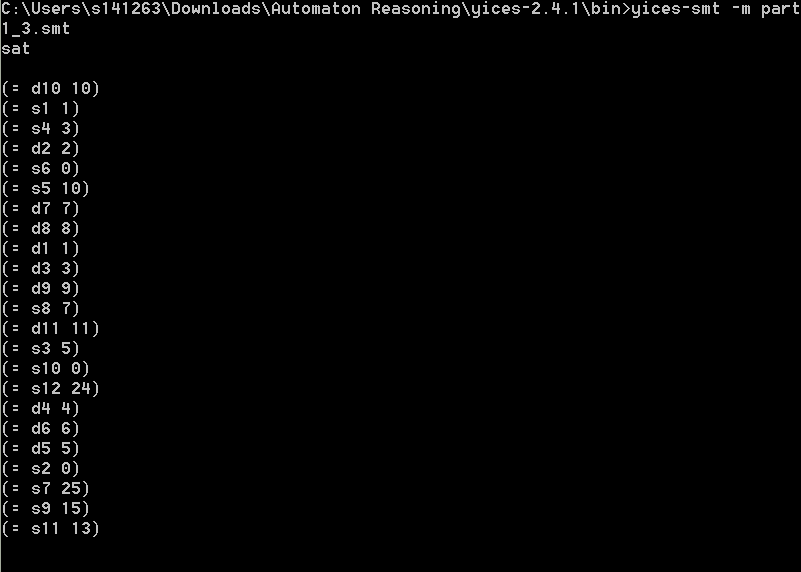
\includegraphics[width=1.0\textwidth]{Part1_3.png}
\end{center}

{\bf Remark:}

\vspace{3mm}

{\bf Generalization:}

\vspace{5mm}

\subsection*{Problem 4}

Seven integer variables $a_{1}$, $a_{2}$, $a_{3}$, $a_{4}$, $a_{5}$, $a_{6}$, $a_{7}$ are given, for which the initial value of $a_{i}$ is $i$ for $i = 1, . . . , 7$. The following steps are defined: choose $i$ with $1 < i < 7$ and execute
\begin{center}
$a_{i} := a_{i−1} + a_{i+1}$,\\
\end{center}
that is, $a_{i}$ gets the sum of the values of its neighbors and all other values remain unchanged. Show how it is possible that after a number of steps there is a number $\geq 50$ that occurs at least twice in $a_{1}$, $a_{2}$, $a_{3}$, $a_{4}$, $a_{5}$, $a_{6}$, $a_{7}$.
\vspace{4mm}

\subsection*{Solution:}

\vspace{3mm}

{\bf Remark:}

\vspace{3mm}

{\bf Generalization:}

\end{document}
